 \documentclass[letterpaper, 10 pt, conference]{ieeeconf}  % Comment this line out
                                                          % if you need a4paper
%\documentclass[a4paper, 10pt, conference]{ieeeconf}      % Use this line for a4
                                                          % paper

\IEEEoverridecommandlockouts                              % This command is only
                                                          % needed if you want to
                                                          % use the \thanks command
\overrideIEEEmargins
% See the \addtolength command later in the file to balance the column lengths
% on the last page of the document

\usepackage[applemac]{inputenc}
\usepackage[T1]{fontenc}
\usepackage{microtype}
\usepackage{amssymb,amsmath}
%\usepackage{amsthm}
\usepackage{mathtools}
\usepackage{color, comment}
\usepackage{graphicx}
\usepackage{textcomp}
\usepackage{gensymb}
\usepackage{times}
\usepackage{mathptmx}
\usepackage{epsfig}
\usepackage{gensymb,bbm}
\usepackage{stmaryrd}



\setcounter{secnumdepth}{4} % how many sectioning levels to assign numbers to
\setcounter{tocdepth}{4}    % how many sectioning levels to show in ToC
\usepackage{mathtools}
\DeclarePairedDelimiter{\ceil}{\lceil}{\rceil}

\newcommand{\convhull}{\mbox{convhull } }
\newcommand{\R}{\mathbb{R} }
\newcommand{\B}{\mathbb{B} }
\newcommand{\Z}{\mathbb{Z} }
\newcommand{\N}{\mathbb{N} }
\newcommand{\conv}{\convhull }


\newcommand{\proj}{\Pi }
\newcommand{\koverc}{\frac{|k_i|}{\|c_i\|} }
\newcommand{\dist}{d}
\newcommand{\supp}{\text{supp}}
\newcommand{\Opt}{\text{Opt} }

\newcommand{\calA}{\mathcal{A}}
\newcommand{\calB}{\mathcal{B}}
\newcommand{\calC}{\mathcal{C}}
\newcommand{\calD}{\mathcal{D}}
\newcommand{\calE}{\mathcal{E}}
\newcommand{\calF}{\mathcal{F}}
\newcommand{\re}{\mathbb{R}}
\newcommand{\sphere}{\text{S}}
\newcommand{\ball}{\text{B}}


\providecommand{\rmj[1]}{{\color{red}#1}}
\providecommand{\com[2]}{\begin{tt}[#1: #2]\end{tt}}
\providecommand{\comrj[1]}{\com{RJ}{\rmj{#1}}}
\providecommand{\comff[1]}{{\small \color{blue} [FF: {#1}]}}

\newcommand{\calH}{\mathcal{H}}
\newcommand{\calI}{\mathcal{I}}
\DeclareMathOperator*{\argmin}{arg\,min}

\newcommand{\cM}{\mathcal{M}}
\newcommand{\calM}{\mathcal{M}}
\newcommand{\calN}{\mathcal{N}}
\newcommand{\calP}{\mathcal{P}}
\newcommand{\calQ}{\mathcal{Q}}
\newcommand{\calR}{\mathcal{R}}
\newcommand{\calS}{\mathcal{S}}
\newcommand{\calU}{\mathcal{U}}
\newcommand{\calV}{\mathcal{V}}

\newcommand{\n}{\mathbb{N}}
\newcommand{\calK}{\mathcal{K}}
\newcommand{\calW}{\mathcal{W}}
\newcommand{\calY}{\mathcal{Y}}
\newcommand{\calX}{\mathcal{X}}
\newcommand{\calZ}{\mathcal{Z}}

 

\newtheorem{remark}{Remark}[section]
\newtheorem{property}{Property}[section]
\newtheorem{theorem}{Theorem}[section]
\newtheorem{lemma}[theorem]{Lemma}
\newtheorem{proposition}[theorem]{Proposition}
\newtheorem{corollary}[theorem]{Corollary}
\newenvironment{definition}[1][Definition]{\begin{trivlist}
\item[\hskip \labelsep {\bfseries #1}]}{\end{trivlist}}




\title{\LARGE \bf
On learning guaranted bounds for black-box/dark data switched systems ;)
}

%\author{ \parbox{3 in}{\centering Huibert Kwakernaak*
%         \thanks{*Use the $\backslash$thanks command to put information here}\\
%         Faculty of Electrical Engineering, Mathematics and Computer Science\\
%         University of Twente\\
%         7500 AE Enschede, The Netherlands\\
%         {\tt\small h.kwakernaak@autsubmit.com}}
%         \hspace*{ 0.5 in}
%         \parbox{3 in}{ \centering Pradeep Misra**
%         \thanks{**The footnote marks may be inserted manually}\\
%        Department of Electrical Engineering \\
%         Wright State University\\
%         Dayton, OH 45435, USA\\
%         {\tt\small pmisra@cs.wright.edu}}
%}

\author{Ay\c{c}a Balkan, Raphael Jungers, Joris Kenanian, Paulo Tabuada% <-this % stops a space
%\thanks{This work was not supported by any organization}% <-this % stops a space
%\thanks{H. Kwakernaak is with Faculty of Electrical Engineering, Mathematics and Computer Science,
%        University of Twente, 7500 AE Enschede, The Netherlands
%        {\tt\small h.kwakernaak@autsubmit.com}}%
%\thanks{P. Misra is with the Department of Electrical Engineering, Wright State University,
%        Dayton, OH 45435, USA
%        {\tt\small pmisra@cs.wright.edu}}%
}


\begin{document}



\maketitle
\thispagestyle{empty}
\pagestyle{empty}


%%%%%%%%%%%%%%%%%%%%%%%%%%%%%%%%%%%%%%%%%%%%%%%%%%%%%%%%%%%%%%%%%%%%%%%%%%%%%%%%
\begin{abstract}

To do - Ay\c{c}a?

\end{abstract}


%%%%%%%%%%%%%%%%%%%%%%%%%%%%%%%%%%%%%%%%%%%%%%%%%%%%%%%%%%%%%%%%%%%%%%%%%%%%%%%%
\section{INTRODUCTION}

As the computational power of the computers has increased, so is the complexity of dynamical systems we can model with them. Today, the industrial dynamical systems does not only consist of simple differential or difference equations; they are multimodal, hybrid, and often contain variety of subcomponents such as lookup tables, delay differential equations, actuation delays and thermodynamic models. The current modeling paradigm is also highly distributed, in the sense that, some of the model subcomponents are developed by different parties and therefore their internal structure is partially, if not completely unknown to the end user.
Hence, it is often virtually impossible to obtain simple analytical formulas for today's industrial scale dynamical system models. However, thanks to the advances in our computational power again, in spite of this increased complexity, for a notable subset of these models we can still efficiently perform simulations. Therefore, it is a natural question to ask whether we can provide formal analyses about certain properties of these systems based solely on the collected simulation data. In this paper, we focus on the analysis of one of the most important properties of dynamical systems in the context of control theory: stability.

%\textcolor{red}{There is no model.
%System are getting more complex, multimodal, lookup tables, thermodynamics, there is a need to ?prove properties about these systems, despite the fact that the modesl are mo complex are partially knowni Subcomponetns come from  different companies and black box.
%We still need to prove properties.
%The most important property in terms of control: stability.
%Even in the case when we have a model the stability is hard, for example Raphael, therefore we shouldn't expect we are gonna do better. The first step towards just based on switched systems. Because these are the very simple class of systems, resoanable it captures many applications.
%Even in the case of linear systems we cannot say anything. Here, we put the example where even the system is linear, we cannot say anything by just looking at the lyapunov functions decrease.}
More formally, given a dynamical system as in:
\begin{equation}\label{eq:dydnamicalsystemGeneral}x_{k+1} = f(k, x_k),
\end{equation}
where, $x_k \in \R^n$, k is index of time. Let $y_k := x_{k+1}$
We ask the following question: \emph{
given N input-output pairs, $(x_1, y_1)$, $(x_2, y_2)$, $\ldots$, $(x_N, y_N)$ such that $y_{k} = f(k, x_k)$, what can we say about the stability of the system \eqref{eq:dynamicalsystemGeneral}?} The answer is immediate when \eqref{eq:dynamicalsystemGeneral} is a linear time-invariant system, since we can simply identify the system by $n$ linearly independent output traces. In this paper, we seek the answer to this question for switched linear systems for which the problem immediately becomes nontrivial. A switched linear systems is in the form:
\begin{equation}\label{eq:switchedSystem}x_{k+1} = A_{\sigma(k)}x_k,\end{equation}
where, $\sigma: \N \to \{1,2, \ldots, m\}$ is the switching sequence and $A_{\sigma(k)} \in \calM$, for all $\sigma$ and $k$. Aside from their theoretical value, switched systems model the behavior of dynamical systems in the presence of known or unknown varying parameters. These parameters can model internal properties of the dynamical system such as uncertainties, look-up tables, values in a discrete register as well as exogenous inputs provided by a controller in a closed-loop control system. 

%To make our reasoning clearer, we introduce the \emph{Lyapunov exponent} of the system \eqref{eq:switchedSystem}, which is a numerical quantity describing its stability.
%\begin{definition} Given a dynamical system as in \eqref{eq:dynamicalsystem} its \emph{Lyapunov exponent} is given by
%$$\rho =\inf{\{r:\,\forall x_0, \exists C\in \re^+: \quad x(0)=x_0 \Rightarrow x(t)\leq Cr^t\}}. $$
%\end{definition}
%Under certain conditions, deciding stability amounts to decide whether $\rho<1.$  In order to understand the quality of our techniques, we will actually try to prove lower and upper bounds on $\rho.$ 
Assessing the stability of nonlinear systems by leveraging simulations has been an active area of research in the recent years. Simulation data has been used in both construction and verification of Lyapunov functions. Topcu et.al. \cite{topcu} and Kapinski et.al. \cite{kapinski} construct Lyapunov function candidates using the simulation traces, however to be able to formally verify the constructed Lyapunov function, they require the knowledge of the full dynamics. In \cite{lazar} and \cite{lazar2} Bobiti and Lazar address this and provide sampling based probabilistic and deterministic guarantees of a given Lyapunov function candidate. The presented method requires the knowledge of how fast the output of the system can change as the initial condition changes, and moreover the number of required samples increases exponentially in the dimension of the state, $n$.

The stability of switched systems closely relates closely to the \emph{joint spectral radius} (JSR) of the matrices appearing in \eqref{eq:switchedSystem}. Under certain conditions deciding stability amounts to deciding whether JSR less than one or not. There has been a lot of work on developing algorithms to approximate this quantity, when the matrices appearing in \eqref{eq:switchedSystem} are known. Therefore, our work is also connected to the identification of switched systems, since once the system \eqref{eq:switchedSystem} is identified one can then apply these well-established results. However, there are two main reasons behind our quest to directly work on input-output pairs and bypassing the identification phase: (1) Even when $\calM$ is known, approximating the JSR is NP-hard \cite{jungers}. (2) Identifying the set $\calM$ is also NP-hard. Therefore, the existing identification techniques can identify $\calM$ up to an approximation error. As a result, how to relate this identification error to an error on the stability of \eqref{eq:switchedSystem} is still nontrivial.

In this paper, we present an algorithm to approximate the JSR of a switched linear system from $N$ input-output pairs. This algorithm provides an upper bound on the JSR with a user-defined confidence level. As the number of samples increases, this bound gets tight. Moreover, we characterize with a closed form expression what the exact trade-off between the tightness of this bound and the number of samples is. In order to understand the quality of our technique, the algorithm also provides a deterministic lower-bound.

The organization of the paper is follows: Section \label{preliminaries} introduces our notation and definitions from the switched linear system literature to present our results, Section \label{problemDefinition} formalizes the problem definition, Section \label{upperBound} provides an algorithm to compute a deterministic lower bound and 
%
%In this paper, we consider discrete-time switched linear systems of the form:
%\begin{equation}\label{eq:dynamicalsystem}x_{k+1} = A_{\sigma(k)}x_k,
%\end{equation}
%where, $x_k \in \R^n$, k is index of time and $\sigma: \N \to \{1,2, \ldots, m\}$ is the switching sequence. Let $y_k := x_{k+1}$. 
%We ask the following question:
%\begin{centering}
%\emph{Given N input-output-matrix pairs, $(x_1, y_1)$, $(x_2, y_2)$, $\ldots$, $(x_N, y_N)$ such that
%\begin{equation}\label{eq:triples}y_{k} = A_{\sigma(k)}x_k,
%\end{equation} for some $\sigma(k),$ what can we say about the stability of the system \eqref{eq:dynamicalsystem}?
%\end{centering}
%The only instance where answer to this question has been clearly shown is for linear time-invariant systems.
%
%Note that if \eqref{eq:dynamicalsystem} is a linear time-invariant system with only one mode, this question is easily answered by observing $n$ linearly independent data points. Switched systems can be used to model the behavior of a system of interest for different values of a parameter that varies. This parameter can represent internal parameters such as model uncertainties, as well as exogenous parameters such as inputs provided by a controller in a closed-loop control system. 


%- Stability analysis of dynamical systems is a challenging task. \\
%- Most methods in literature rely on knowing the model. Cite \\
%- How to make the case about the assumption of switched linear yet, we don't construct a model? Here cite
%something that says that this is a hard problem in general. (What is the relationship between switching linear regression)
%- Here we present stability analysis from data, this is easy for linear systems. We present something for switch linear.



%I can refer to the condition number paper?

%%%%%%%%%%%%%%%%%%%%%%%%%%%%%%%%%%%%%%%%%%%%%%%%%%%%%%%%%%%%%%%%%%%%%%%%%%%%%%%%

\section{PRELIMINARIES AND PROBLEM DEFINITION}

We consider the usual Hilbert finite normed vector space $(\R^n,\ell_2)$, $n \in \mathbb{N}_{> 0}$, $\ell_2$ the classical euclidean norm. We denote a unit ball in $\R^n$ with $\ball$ and unit sphere in $\R^n$ of radius $r$ as $\sphere$. We only denote the radius $r$ explicitly as in $\ball_r$ and $\sphere_r$, when $r$ is different than $1$. We denote the set of real symmetric matrices of size $n$ by $\mathbb{S}^n$, and the set of linear functions in $\R^n$ by $\mathcal{L}(\mathbb{R}^n)$. We denote the ellipsoid described by the matrix $P \in \mathbb{S}^n$ as $E_P$. We denote the homothety of ratio $\lambda$ by $\calH_{\lambda}$.

We denote by $M$ the set $\{1,2,\dots,m\}$, ($m \in \N_{>0}$) and consider a switched linear system of modes $\calM = \{A_1, A_2,\dots, A_m\} \subset \R^{n \times n}$ indexed by $M$. We observe the system: 
\begin{equation}\label{eq:dynamicalsystem}x_{k+1} = A_{\sigma(k)}x_k,
\end{equation}
where, $x_k \in \R^n$, k is index of time and $\sigma: \N \to M$ is the switching sequence. Let $y_k := x_{k+1}$. 
We assume that we only know the number of modes $m$, the input $x_k$ and the output $y_k$ at each time $k$. We ignore what are the matrices and the index of the matrix which is applied at every time. We consider the following problem.

\begin{centering}
\emph{Given N input-output-matrix pairs, $(x_1, y_1)$, $(x_2, y_2)$, $\ldots$, $(x_N, y_N)$ such that
\begin{equation}\label{eq:triples}y_{k} = A_{\sigma(k)}x_k,
\end{equation} for some $\sigma(k),$
 (but not necessarily $x_{k+1}=y_k$) how can we decide if the switching system is stable?}
\end{centering}

To make our reasoning clearer, we introduce the \emph{Lyapunov exponent} of the system, which is a numerical quantity describing its stability.
\begin{definition}   Given a dynamical system as in \eqref{eq:dynamicalsystem} its \emph{Lyapunov exponent} is given by
$$\rho =\inf{\{r:\,\forall x_0, \exists C\in \re^+: \quad x(0)=x_0 \Rightarrow x(t)\leq Cr^t\}}. $$
\end{definition}
Under certain conditions \comrj{to be epxplicited}, deciding stability amounts to decide whether $\rho<1.$  In order to understand the quality of our techniques, we will actually try to prove lower and upper bounds on $\rho.$ 



\subsection{Examples}

Many observations, coherent with the existence of a quadratic Lyapunov function, do not mean much, even for linear systems. We can see for the simple linear system
\[
\dot{x}(t) =
\begin{bmatrix}
-2 & 0\\
0 & 0.1
\end{bmatrix} 
x(t)\]
that by sampling on the unit circle, as long as we do not pick points from the blue areas, we will observe a contraction of the points. Nevertheless, all the trajectories with initial condition $x \in \R^2 - \{(\lambda,0), \lambda \in \R\}$ will eventually diverge.


\begin{figure}[h]
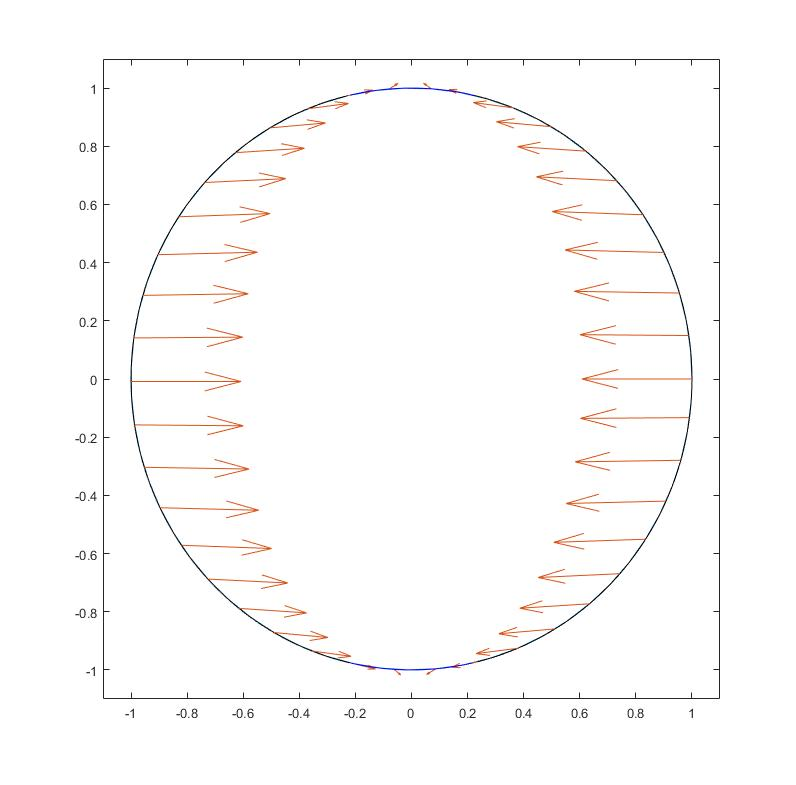
\includegraphics[scale=0.25]{example.jpg}
\end{figure}


\subsection{Assumptions}
It is clear that one has to pose assumptions on the dynamical system studied in order to be able to infer stability properties from the observations of samplings of its dynamics: one can easily build nonlinear systems such that the Euclidean norm of most points is dramatically decreased by one iteration of the system, but however the system is unstable.  Even more, as we have seen in Example \ref{ex:bad}, there are linear systems that exhibit this property.  One goal of this work is to understand what are the important properties that a system should enjoy, and what type of guarantees they could imply in terms of stability.  We list here a few properties that are going to be studied in this work.

\begin{property}\label{property:poly}
The dynamical system is a polynomial of bounded degree $d.$
\end{property}
\begin{property}\label{property:homogeneity}
The dynamical system is a homogeneous function of the statespace: $$x'_0=\lambda x_0 \Rightarrow x'(t)=\lambda x(t). $$
\end{property}
\begin{property}
The dynamical system is a switching linear system

\begin{equation}\label{switchedSystem}x_{k+1} = A_{\sigma(k)}x_k,
\end{equation}
where, $x_k \in \R^n$, k is index of time and $\sigma: \N \to \{1,2, \ldots, m\}$ is the switching sequence.  This is the first example we'll study.
In this case the Lyapunov exponent is known as the Joint Spectral Radius of the set of matrices, which can be alternatively defined as follows:
\begin{definition}  \cite{jungers_lncis} Given a set of matrices $\cM \subset \re^{n\times n},$ its \emph{joint spectral radius} (JSR) is given by
$$\rho(\cM) =\lim_{t\rightarrow \infty} \max_{i_1,\dots, i_t}\{||A_{i_1} \dots A_{i_t}||^{1/t}: A_i\in\cM\}. $$
\end{definition}
\begin{remark}
 Note that one can scale the problem because the JSR is homogeneous:
$$\rho(\cM/\lambda)=\rho(\cM)/\lambda\, \forall \lambda>0, $$ and $\cM/\lambda$ can be studied by studying the scaled inputs $$(x_t, y_t/\lambda,\sigma(t)).$$
\end{remark}
\end{property}
\begin{property}\label{property:convpres}
 The function $f$ is \emph{convex-preserving,} meaning that for any set of points $X=\{x_i\},$ one has
$$ f(\conv{X})\subset \conv\{f(x_i)\}. $$
\end{property}
We do not know until now whether there are many functions that have the above property, or even whether there are non-linear functions that have it. It turns out that switching linear systems have this property. There is a similar property, that seems to imply (something similar to) the previous one:
\begin{property}\label{property:kconvexity} \cite{VaB:96}Let $K$ be a (convex solid pointed) cone. The function $f$ is \emph{$K$-convex,}  meaning that \begin{itemize} \item it is $K$-monotone: for any $x,y\in K,$ $$x\preceq_K y \Rightarrow f( x )\preceq_K  f(y)$$ \item for any $x,y\in \re^n,$ and $\lambda \in \re,$ $f(\lambda x + (1-\lambda)y)\preceq_K \lambda f(x) + (1-\lambda)f(y).$ \end{itemize}
\end{property}



\section{A lower bound}



For the lower bound, we will leverage the following theorem from the switching system literature.

\begin{theorem}\cite[Theorem 2.11]{jungers_lncis}\label{thm:john}
For any bounded set of matrices such that $\rho(\cM)<1/\sqrt(n),$ there exists a Common Quadratic Lyapunov Function (CQLF) for $\cM,$ that is, a $P\succeq 0$ such that $$\forall A\in \cM,\, A^TPA\preceq P. $$
\end{theorem}

\comrj{We can probably generalize this result.  What is needed is a Converse Convex Lyapunov Theorem: stability implies the existence of a convex (or, quasiconvex, it should suffice) Lyapunov function.  Maybe we should use Mircea's result \cite{geiselhart2014alternative}.  This would be nice per se, I think.}
%
%\begin{theorem}{jungers_lncis}\label{thm:john}
%If a For any bounded set of matrices such that $\rho(\cM)<1/\sqrt(n),$ there exists a Common Quadratic Lyapunov Function (CQLF) for $\cM,$ that is, a $P\succeq 0$ such that $$\forall A\in \cM,\, A^TPA\preceq P. $$
%\end{theorem}

The existence of a CQLF for our (potentially scaled) blackbox system is certainly something we can check: after collecting $N$ observations, one can solve the following optimization problem efficiently. 

\begin{eqnarray}
\nonumber \mbox{min}&&\lambda\\
 s.t.& & \label{eq:lowerbound} \forall 1\leq i \leq N,\ (y_i^T P y_i)/\lambda^2 \leq x_i^TPx_i\\
\nonumber && P \succeq 0.
\end{eqnarray}
Indeed, when $\lambda $ is fixed, the problem is a set of LMIs, and $\lambda $ can be optimized by bisection.

\begin{theorem}
Let $\lambda^*$ be the minimum $\lambda$ such that \eqref{eq:lowerbound} above has a solution.  If $\lambda^*<\infty,$ one has $$\rho(\cM) \geq \lambda^*/\sqrt(n) .$$
\end{theorem}
\begin{proof}
Just apply Theorem \ref{thm:john} to $\cM /(\lambda^*-\epsilon),$ for any $\epsilon>0.$ Since this latter set has no CQLF, we obtain that $\rho(\cM)/\lambda^*\geq 1/\sqrt{n}.$
\end{proof}


This result could be improved in several ways: first, it is classical in the JSR literature to replace the CQLF with a SOS polynomial of degree $2d,$ $d>1.$ this narrows the $1/\sqrt(n)$ accuracy factor, up to one when $d\rightarrow \infty.$  \comrj{this is not 100 \% clear but interesting: if we take a too large degree for a fixed number of points, we will always find a very small lower bound! Nevertheless I hope that it will be easy to understand how increasing the degree can improve the accuracy, and anyway there are interesting things there.}


\section{An upper bound}
\comrj{it is not clear how this upper bound can be useful for switching systems, because we need to know the modes here, and then the system can be easily identified, but maybe for general $f$ it is? Or, maybe it's possible to reuse the same type of ideas without knowing the nodes?}
It is classical to try to upper bound the JSR by constructing a polytope norm \cite{GP11}, defined by a set of points $X=\{x_i:\, i=1,\dots,N\}$ satisfying the following property:
if $$ (A_i/\lambda) \convhull{(X\cup -X)} \subset \convhull{(X\cup -X)},\quad \forall A_i\in \cM$$ then, $$\rho(\{A_1,\dots,A_m\}) \leq \lambda.$$ This can easily be checked by verifying that $$\forall x\in X,\, \forall A\in \cM,\, Ax/\lambda \in \convhull{(X\cup -X)}, $$ that is, by verifying the property only for the vertices of the polytope.

Now, in our situation, we would like to address situations where we do not command what matrix is applied, and/or which point in the state space is selected for the next triple $(x_t, y_t,\sigma(t)).$  It turns out that this slight difference with the `classical JSR computation' can be accounted for:

\begin{theorem}
Suppose that one has m sets of observations $$S_j=\{(x_{j,1}, y_{j,1}),\dots, (x_{j,t_j}, y_{j,t_j})\}$$ as in \eqref{eq:triples}, and denote $$X_j=\{x_{j,t}:t=1,\dots,t_j\},$$ then the solution of the following optimization problem
\begin{eqnarray} \label{eq:upperbound}
\mbox{min}&&\lambda\\
\nonumber s.t.& &\forall i,t,\quad y_{i,t}/\lambda \in \bigcap_{1\leq j \leq m} \convhull{(X_j\cup -X_j)}
\end{eqnarray}
is a valid upper bound on $\rho(\cM).$
\end{theorem}
\begin{proof}
Let us denote $S=\bigcap_{1\leq j \leq m} \convhull{(X_j\cup -X_j)}.$  Fix any feasible $\lambda$ for \eqref{eq:upperbound}. Since for all $j:\ 1\leq j \leq m$ $$S \subset \convhull{(X_j\cup -X_j)}$$ and $$ (A_j/\lambda)\  \convhull{(X_j\cup -X_j)} \subset S,$$ we have that $$ (A_j/\lambda) S\subset S\, \quad \forall 1\leq j \leq m, $$ and this proves that $\rho \leq \lambda.$
\end{proof}

It is not difficult to see that the above bound could be improved further: indeed, it relies on sets of points $X_i,$ for which we know the image by the matrix $A_i.$ However, if we know that $A_ix=y,$ then, we know of course that, for any real number $\lambda,$  $ A_i(x/\lambda)=y/\lambda.$ In other words, we can scale the couples $(x_{j,i},y_{j,i})$ above by any factor $\lambda,$ and this would still give a valid upper bound.  Thus, one could try to optimize over this scaling factors in order to get the best possible upper bound.
This gives the following optimization problem:

\begin{theorem}
Suppose that one has m sets of observations $$S_j=\{(x_{j,1}, y_{j,1}),\dots, (x_{j,t_j}, y_{j,t_j})\}$$ as in \eqref{eq:triples}, and denote $$X_j=\{x_{j,t}:t=1,\dots,t_j\},$$ then the solution of the following optimization problem
\begin{eqnarray} \label{eq:upperbound2}
\mbox{min}_{\lambda,\lambda_{j,t}} &&\lambda\\
\nonumber s.t.& &y_{j,t}/(\lambda \lambda_{j,t}) \in \bigcap_{1\leq j \leq m} \convhull{(\{x_{j,t}/\lambda_{j,t},-x_{j,t}/\lambda_{j,t}\})}.
\end{eqnarray}
is a valid upper bound on $\rho(\cM).$
\end{theorem}

\subsection{A heuristic to improve the upper bound}

The above program \eqref{eq:upperbound2} aims at finding scaling factors of the couples $(x_{j,i},y_{j,i})$ so as to minimize the upper bound.  Intuitively, there is an optimal scaling factor which can be defined as follows: let us denote $||\cdot||_*$ the \emph{extremal norm} of the set of matrices ; that is, the norm satisfying \begin{equation}\label{eq:extremal}\forall x\in \re^n \quad  \max_{A_i \in \cM}||A_ix||_*=\rho ||A_i||_*. \end{equation}  Such a norm always exists for any bounded set of matrices $\cM$, provided that the matrices do not share a common invariant subspace \cite[Section 2.1.2]{jungers_lncis} (if they do, this does not change our discourse, since there exists in any case a norm satisfying \eqref{eq:extremal}, with $\rho$ replaced by $\rho+\epsilon,$ for any $\epsilon>0$).

Suppose that every set $(X_j)$ is the complete unit ball $B_*=\{x:||x||_*=1\}.$
Then, by the definition \eqref{eq:extremal} of $||\cdot ||_*$,we have that $$y_{j,t}/\rho \in \bigcap_{1\leq j \leq m} \convhull{(X_j\cup -(X_j))}, $$ because $ \convhull{(X_j)\cup -(X_j)}=B_*,$
and by \eqref{eq:upperbound} one has a perfect upper bound on $\rho.$  This suggests to scale the $x_{j,t}$ with an approximation of the extremal norm.  Now, remark that Equation \eqref{eq:lowerbound} is precisely aiming at approximating the Definition \eqref{eq:extremal} of an extremal norm.  Of course, it is only an approximation, because it only takes into account the finite number of points available, and restricts the possible norms to ellipsoidal ones.  However, if no other way is available for optimizing \eqref{eq:upperbound}, it is hopeful that this approximation could work well.  Summarizing, we propose to fix \begin{equation}\label{eq:heuristic}\lambda_{j,t}=\sqrt{x_{j,t}^TPx_{j,t}},\end{equation} where $P$ is the solution of \eqref{eq:lowerbound} as a heuristic solution to \eqref{eq:upperbound2}. \comrj{again we might have to trash all the above because knowing the modes allows us to identify the matrices, but it seems that there are good ideas to use for more general models...}

\section{An upper bound with a level of confidence.}\label{section-campi}
In this section we suppose that we do not observe the modes, but only the pairs $(x_k,y_k).$
Our goal here is to improve the upper bound by paying a little bit of uncertainty. Also, it allows us to provide a bound even if we do not know the modes. The idea is that if we have a polytope that is contracted for all our observed pairs $(x,y),$  it is not enough to imply stability, because we observed only some possible behaviours of the dynamics.  However, suppose that we observed that the $\lambda-$contraction of the polytope $\calP$ is satisfied for many values of $x,$ then, it is tempting to extrapolate our observation, and claim that (noting $y=f(x) $ as always),


\begin{equation}\label{eq:polytopic norm}
\forall{x} \in \re^n \mbox{ s.t. } Cx\leq b \Rightarrow \quad Cy/\lambda \leq b,
\end{equation}

where $C,b$ is the canonical representation of the polytope $\calP.$ 

Similarly, if we observed the $\lambda-$contraction for the quadratic Lyapunov function $x^\top P x,$ it is tempting to generalize to the whole state space:

\begin{equation}\label{eq:cqlf}
\forall{x} \in \re^n,\,  (y^T P y)/\lambda^2 \leq x^TPx.
\end{equation}
Both equations imply that $\rho\leq \lambda.$

Unfortunately, the true observations only imply that these inequalities are valid for a few points $x_i,$ not for the whole statespace. However we will use classical probability results to bridge the gap between our observations, and a stability guarantee for the complete statespace. Observe that a priori this gap is not negligible, and for instance in Example \ref{ex:bad} one can see that there exists a quadratic function which satisfies the Lyapunov equation for almost all the points, but yet, almost all the trajectories are unstable.
We recall a classical result on optimization with a sampled subset of constraints:
\begin{theorem} \cite{calafiore2005uncertain,calafiore2006scenario}\label{thm:campi}
For any convex program, with a measure on the constraints, in any fixed dimension $n,$ and for any $0 < \epsilon,$ $ \beta< 1,$ there exists a number $N(\epsilon, \beta)$ such that, if one samples $N$ constraints, then, with probability larger than $\beta,$ the solution of the optimization program with these $N$ constraints satisfies a subset of the full constraints set of measure at least $1-\epsilon.$
\end{theorem}

We first consider a simpler version of our theorem, which corresponds to the case $n=0$ above, and where the polytope is fixed a priori.  This is clearly conservative but is there for the sake of clarity.
\comrj{We are trying to prove something as clean as possible... probably this simpler version will be removed later.
%It seems crucial that there is a switching phenomenon here, because in the other case, one could just use the generalized convexity Assumption \ref{property:convpres} in order to prove stability without paying some confidence.  In the future, we plan to understand what other types of situations necessitate to pay a little of confidence in order to deduce stability (digital controller with hidden variables?).
}
\begin{theorem}
Consider a polytope\footnote{all our polytopes are supposed to be symmetric wrt the origin, so that they can be considered as the unit ball of a norm.} $$\calP_{C,b}=\{x: Cx\leq b\}$$ which is fixed a priori.  Consider a black-box switching system and $N$ couples (randomly, uniformly sampled) of its dynamics as in \eqref{eq:triples}.   Suppose that the polytope is invariant for all the observations (one can always scale the set of matrices and apply the theorem to the scaled version).  That is, if the observed couples $(x,y)$ are scaled so that $x$ belongs to the boundary of the polytope, one has \begin{equation}\label{eq:invpoly} Cy\leq b.\end{equation} Then, for any factor $1<\delta,$ one can compute the level of confidence $\beta$ such that $\rho<\delta.$  
% denote $\gamma(P,\epsilon)$ the largest $\gamma$ such that $\gamma^2y_i^TPy_i\leq x_i^TPx_i$ 

\end{theorem}

\begin{proof}


Let us fix $\delta>1.$  Define $\epsilon$ as the smallest measure of a set \begin{equation}\label{eq:epsilonvsdelta} X\subset \partial \calP \mbox{ s.t. } \delta^{-1} = \sup{\{d: d \calP \subset \conv{\partial \calP\setminus X}\} }. \end{equation}
In the equation above, $\partial$ represents the boundary of a set, and by measure, we mean the uniform measure on the Euclidean ball $B$ (more precisely, $\mu(X)= \mu'(\{x\in B: \exists x'\in X, \lambda \in \re^+; x = \lambda x'\});$ and $\mu'$ is the uniform measure on the Euclidean ball).

 Since Equation \eqref{eq:invpoly} does not contain any variable, it is a trivial application of Theorem \ref{thm:campi}, (or an application of first principles in probability) that, if the (scaled) vectors $x$ are sampled randomly (say, on the unit sphere), and if we have $N$ of these observations all of them satisfying  \eqref{eq:invpoly}, then we can claim that the measure of points $x$ that violate  \eqref{eq:invpoly} (more precisely, the points $x$ such that, denoting $ \hat x$ the scaled vector such that $\hat x$ belongs to the boundary of the polytope, we have that the image $y=f(\hat x)$ does not satisfy $ Cy\leq b$) is smaller than $ \epsilon$ with confidence $1-(1-\epsilon)^N.$   Indeed, suppose by contradiction that the measure is $\epsilon ' \geq \epsilon.$ Then, the probability that our $N$ samples satisfy \eqref{eq:invpoly} is equal to $(1-\epsilon')^N \leq (1-\epsilon)^N .$  Thus, the level of confidence of our Hypothesis that only an $\epsilon$ measure of points $x$ violate  \eqref{eq:invpoly} is $1-(1-\epsilon)^N.$

Summarizing, the equation above means that with confidence $\beta := 1-(1-\epsilon)^N$, one has that \eqref{eq:invpoly} is satisfied for all $x\in \R^n,$ except for a set of measure $\epsilon.$   Let us denote $S_\epsilon$ this set of violated constraints.  That is, $$f(\partial\calP\setminus S_\epsilon) \subset \calP.$$  By our assumption \ref{property:convpres}, $$f( \convhull (\partial\calP\setminus S_\epsilon) \subset \convhull (f(\partial\calP\setminus S_\epsilon)).$$  Combining the above two equations with our choice of $\epsilon$ in Equation \eqref{eq:epsilonvsdelta},  we have that  
$$f( \convhull (\partial\calP\setminus S_\epsilon) \subset \convhull (\partial\calP\setminus S_\epsilon)/\delta,$$

and so $\rho\leq \delta$ with confidence $\beta := 1-(1-\epsilon)^N.$
 
\end{proof}


\subsection{the stronger version of the theorem}
\comrj{This stronger version looks for an ellipsoid. We believe that everything is correct below too, but there's a little catch in the 'one can compute': for the moment we do not really know how to algorithmically compute $\epsilon$ like in the proof above, essentially because we have ellipsoids (but note that even for the polytope above, everything is not crystal clear yet).}
\begin{theorem}
Consider a black-box switching system and $N$ samples of its dynamics as in \eqref{eq:triples}. Consider the optimal solution $(\lambda^*,P)$ which minimizes $\lambda$ in \eqref{eq:lowerbound}. For any factor $1<\delta,$ one can compute the level of confidence $\beta$ such that $\rho<\delta\cdot\lambda^*.$ 
% denote $\gamma(P,\epsilon)$ the largest $\gamma$ such that $\gamma^2y_i^TPy_i\leq x_i^TPx_i$ 

\end{theorem}

\begin{proof}


Let us fix $\delta>1$ and denote $E_P$ the ellipsoid described by $P$ (i.e., $\{x:x^TPx= 1\}$), and denote $\epsilon$ such that for any subset $S_\epsilon$ of measure $\epsilon,$ 
$$ E_{\delta^2P} \subset  \convhull (E_P\setminus S_\epsilon) .$$ 
  
	(\comrj{this is where we still have to find a solution} First prove that the worst-case $S_\epsilon$ should be one single connected set, then, it should be centered around the longest axis of the ellipsoid.) \comrj{Alternatively, can't we simply rescale the state space so that the ellipsoid becomes a sphere? Then, we know how to compute the $\epsilon.$ We hope that this would come at the only price of increasing the measure of the points we miss, because we know how we distorded the measure.  To be checked, fingers crossed.}
	
	
Now, denoting $N$ the number of observations available, compute $0< \beta< 1$ such that $$N=N(\epsilon,\beta)$$ in Theorem \ref{thm:campi} above. 

Summarizing, the equation above means that with high probability, one has that \eqref{eq:lowerbound} is satisfied for all $x\in \re^n,$ except for a set of measure $\epsilon.$  Let us denote $S_\epsilon$ this set of violated constraints.  Thus, $$(\cM/\lambda^*) \convhull (E_P\setminus S_\epsilon) \subset \convhull (E_P\setminus S_\epsilon).$$  Now, by definition of $\epsilon,$ one has

$$ E_{\delta^2P} \subset  \convhull (E_P\setminus S_\epsilon) ,$$ and so
$$
(\cM/\delta \lambda^*) \convhull (E_P \setminus S_\epsilon) \subset \convhull (E_P\setminus S_\epsilon).$$

%Moreover, except for $x\in S_\epsilon$, one has $$(y^T P y)/(\lambda^2 *\gamma^2) \leq x^TPx/\gamma^2,$$  N

Then, $\delta\lambda$ is un upper bound on $\rho,$ with a confidence $\beta.$ 
\end{proof}

\section{Campi's preliminaries}

 Let us consider $X = \sphere \times M$ the Cartesian product of the unit sphere $\sphere$ with $M$. Every element of $X$ can be written as $x = (s_x, k_x)$ with $s_x \in \sphere$ and $k_x \in M$. For notational simplicity, we drop the subscript $x$ whenever it is clear from the context.

We define the projections:
$$\pi_{\sphere}: \sphere \times M \rightarrow \sphere, (s,k) \mapsto s$$
$$\pi_M: \sphere \times M \rightarrow M, (s,k) \mapsto k.$$

%It is well-known that $\sphere$ is a $n-1$ embedded submanifold of $\mathbb{R}^n$, and can thus be seen as an image of an atlas (collection) of smooth maps $\phi_i: U \to \sphere$, $U \in \mathbb{R}^n$ called charts. It has the topology inherited from its ambient space $\mathbb{R}^n$. If $\mathbb{R}^n$ is provided with a $\sigma$-algebra $\Sigma$, this parametrization also induces a $\sigma$-algebra on $\sphere$, $\Sigma_{\sphere}$. Hence, a measure $\mu$ on the measurable space $(\mathbb{R}^n, \Sigma)$ defines a measure $\mu_{\sphere}$ on the measurable space $(\sphere, \Sigma_{\sphere})$. This measure can be seen as push-forward $\phi_{i*}(\mu)$ of $\mu$ by the charts, i.e., $\phi_{i*}(\mu)(A) = \mu(\phi_i^{-1}(A))$ for any $A \in \Sigma_{\sphere}$. 

We consider the classical unsigned and finite uniform spherical measure on $\sphere$, commonly denoted by $\sigma^{n-1}$. It is associated to the spherical Borelian $\sigma$-algebra and is derived from the Lebesgue measure (a measure of subset of the sphere will be related to the measure of the sector of the unit ball it induces).

More formally, we will have $\mathcal{B}_{\sphere}$ with $\calA \in \mathcal{B}_{\sphere}$ if and only if the sector $t \calA$, $t \in [0,1]$ is in $\mathcal{B}_{\mathbb{R}^n}$. The spherical measure $\sigma^{n-1}$ is defined by
$$\forall\ \calA \in \mathcal{B}_{\sphere}, \sigma(A) = \frac{\lambda(tA)}{\lambda(B)}. $$
We can notice that $\sigma^{n-1}(\sphere) = 1$.

We assume from now that $\sphere$ is provided with $(\mathcal{B}_{\sphere},\sigma^{n-1})$ and that $M$ is provided with the classical $\sigma$-algebra associated to finite sets: $\Sigma_M = \wp(M)$, where $\wp(M)$ is the power set of $M$.

We consider an unsigned finite measure\footnote{Recall that the support of a measure $\mu$ defined on a measurable space $(X, \Sigma)$ is $\text{supp}(\mu) = \overline{\{A \in \Sigma | \mu(A) > 0 \}}$} $\mu_M$ on $(M, \Sigma_M)$ with $\text{supp} (\mu_M) = M$. In other words, $\forall\,k \in M$, $\mu_M(\{k\})  > 0$.

%[Comment: basically we force here the measure we take on the set of mode indices to be nonzero for every mode].

We denote the product $\sigma$-algebra $\mathcal{B}_{\sphere} \bigotimes \Sigma_M$ engendered by $\mathcal{B}_{\sphere}$ and $\Sigma_M$: $\Sigma = \sigma( \pi_{\sphere}^{-1}(\mathcal{B}_{\sphere}),  \pi_{M}^{-1}(\Sigma_M))$. On this set, we define the product measure $\mu = \mu_{\sphere} \otimes \mu_M$ which is an unsigned finite measure on $X$.

\section{Campi}

We are interested in solving the following optimization problem for a given $\gamma \in (0,1)$:
\begin{equation}
\label{eqn:campiOpt0}
\begin{aligned}
& \text{find} & & P \\
& \text{subject to} 
&  & (A_is)^TP(A_is) \leq \gamma^2 s^TPs, \quad \forall i = \{1,2, \ldots, m\},  \forall\, s \in \sphere,\\
& && P \succ 0. \\
\end{aligned}
\end{equation}
Note that if $P$ is a solution to \eqref{eqn:campiOpt0}, then so is $\alpha P$ for any $\alpha \in \R_{> 0}.$Therefore, we can rewrite \eqref{eqn:campiOpt0} as the following optimization problem:

\begin{equation}
\label{eqn:campiOpt01}
\begin{aligned}
& \text{find} & & P \\
& \text{subject to} 
&  & (A_ks)^TP(A_ks) \leq \gamma^2 s^TPs, \quad \forall i = \{1,2, \ldots, m\},  \forall\, s \in \sphere,\\
& & & P \succeq I.
\end{aligned}
\end{equation}

We define the linear isomorphism $\Phi$ as the natural mapping \mbox{$\Phi: \mathbb{R}^{\frac{n(n+1)}{2}} \to \mathbb{S}^n$.} Using this mapping, for a fixed $\gamma \in (0, 1]$ we can rewrite \eqref{eqn:campiOpt01} as:

\begin{equation}
\label{eqn:campiOpt1}
\begin{aligned}
& \text{find} & & p \\
& \text{subject to} 
& & f(p,x) \leq 0, \forall x \in X.
\end{aligned}
\end{equation}
where $f(p,x) = \max(f_1(p, x), f_2(p))$, and 
\begin{eqnarray*}
f_1(p,x) &:=& (A_ks)^T\Phi(p)(A_ks) - \gamma^2 s^T\Phi(p)s \\
f_2(p) &:=& \lambda_{\max}(\Phi(-p)) +1.
\end{eqnarray*}

%$f(p, \xi)$ is defined as in:
%\begin{equation}\label{eqn:objFunction}f_\gamma(p, x) = \max\left((A_is)^T\Phi(p)(A_is) - \gamma x^T\Phi(p)x,\lambda_{\max}(\Phi(p)) - t, \lambda_{\max}(\Phi(-p)) +1\right).\end{equation}

\begin{proposition}The optimization problem \eqref{eqn:campiOpt1} is convex.
\end{proposition}

\begin{proof}The function $f_1(p,x)$ is clearly convex in $p$ for a fixed $x \in X$. The function 
$\lambda_{max}: \mathbb{S}^n \to \R$ maps a symmetric positive matrix to its maximum eigenvalue. It is well-known that the function $\lambda_{\max}$ is a convex function of $P$. \cite{boyd}. This means that, $p \mapsto \Phi(\lambda_{\max}(p))$ is convex in $p$. Moreover, maximum of convex functions is also convex, which shows that $f(p, x)$ is convex in $p$.
\end{proof}

Note that the optimization problem \eqref{eqn:campiOpt1} has infinitely many constraints. We next consider the following optimization problem where we sample $N$ constraints of \eqref{eqn:campiOpt1} independently and identically with the probability measure
$\mathbb{P}(A) = \frac{\mu(A)}{\mu(X)}, \forall\, A \in \Sigma$, where $N \geq d+1$, and $d := \frac{n(n+1)}{2}$. We denote this sampling by $\omega:=\{x_1, x_2, \ldots, x_N\} \subset X$, and obtain the following convex optimization problem $\Opt(\omega)$: 

\begin{equation}
\label{eqn:campiOpt2}
\begin{aligned}
& \text{find} & & p \\
& \text{subject to} 
& & f(p, x) \leq 0, \forall x \in \omega. \end{aligned}
\end{equation}

Let $p^*(\omega)$ be the solution of $\Opt(\omega)$. We are interested in the probability of $p^*(\omega)$ violating at least one constraint in the original problem \eqref{eqn:campiOpt1}. Therefore, we define constraint violation property next.

\begin{definition}[Constraint violation probability \cite{campi}] The constraint violation probability is defined as:
\begin{equation*}
\calV^*(\omega)=
    \begin{cases}
      \mathbb{P}\{x \in X: f(p^*(\omega), x) > 0\} &\text{if}\,\, \omega \in X^{N*},\\
      1, & \text{otherwise}
    \end{cases}
\end{equation*}
where $X^{N*}:=\{\omega \in X^N: \text{the solution of $\Opt(\omega)$ exists}\}$. 
Note that, since we have $\mathbb{P}(A) = \frac{\mu(A)}{\mu(X)}$, we can rewrite this as:
\begin{equation*}
\calV^*(\omega)=
    \begin{cases}
      \frac{\mu\{x \in X: f(p^*(\omega), x) > 0\}}{\mu(X)} &\text{if}\,\, \omega \in X^{N*},\\
      1, & \text{otherwise}
    \end{cases}
\end{equation*}
\end{definition}

We make the following assumptions on the problem $\Opt(\omega)$:
\begin{enumerate}
\item \label{assumption1} Uniqueness of solution: Note that this can be enforced by adding a tie-break rule of at most $\frac{n(n-1)}{2}$ convex conditions discriminating our solutions. 
\item \label{assumption2} Nondegenaracy: with probability $1$, there is no redundancy in the constraint obtained from the sampling. 
%We can notice that a constraint obtained for a point $(s, k)$ gives us a constraint also on the point $(-s, k)$, and that a set of constraints containing some redundancy in them will be a set of constraints obtained from samples for a same mode. Now, let assume we consider for a fixed mode of index $k$ a nondegenerate sample of points $\{x_1, \dots, x_i\}$. Then if $x_{i+1} \notin \{(\pm s_{x_j},k), \ j \in \{1, \dots, i\} \}$ (which is a set of measure zero), the constraint obtained from $x_{i+1}$ is not redundant. Indeed, the mode of index $k$ might have all its eigenvalues but one with norm lower than $1$, and $x_{i+1}$ might be in the eigenspace of the latter eigenvalue (thus the constraint given by $x_{i+1}$ will be violated). Then, by considering the shortest distance between $x_{i+1}$ and the other points of the sample, we can choose for this eigenvalue a value close enough to $1$ (while being strictly greater than $1$) such that the constraints relative to the other points will still be satisfied.
\end{enumerate}

The following theorem from \cite{campi} explicitly gives a relationship between $V^*(\omega)$ and $N$, $n$.
\begin{theorem}[from \cite{campi}]\label{thm:campi}Consider the optimization problem $\Opt(\omega)$ given in \eqref{eqn:campiOpt2}. Let Assumption \ref{assumption1} and Assumption \ref{assumption2} hold. Then, for all $\epsilon \in (0,1)$ the following holds:
\begin{equation*}\mathbb{P}^N\{\{\calV^*(\omega) \leq \epsilon\} \cap X^{N*}\} \geq 1- \sum_{j=0}^{d} \binom{N}{j}\epsilon^j (1-\epsilon)^{N-j}.\end{equation*}
\end{theorem}

Note that $\epsilon=1-I_{\beta}^{-1}(N-d, d+1)$ and can be interpreted as the ratio of the measure of points in $X$ that might violate at least one of the constraints in \eqref{eqn:campiOpt01} to the measure of all points in $X$.

We now state our main theorem, which is based on Theorem \ref{thm:campi} and devote the next section to proving it step by step. We denote by $\gamma^*$, the optimum value of the following optimization problem:
\begin{equation}
\begin{aligned}
& \min_{P, \gamma} & & \gamma \\
& \text{subject to} 
&  & (A_is)^TP(A_is) \leq \gamma^2 s^TPs, \quad \forall i = \{1,2, \ldots, m\},  \forall\, s \in \sphere,\\
& && P \succ 0. \\
\end{aligned}
\end{equation}

\begin{theorem}[Main Theorem] \label{thm:mainTheorem} For any $\eta > 0$, given $N \geq n+1$ and $\beta \in [0,1)$, we can compute $\delta < \infty$ such that with probability at least $\beta$, $\rho \leq \delta (1 + \eta) \gamma^*$. Moreover, as $N \to \infty$, $\delta \to 1$.
\end{theorem}

\section{Proofs measure}

For a given sampling $\omega \in X^{N*}$, let $V:=\{x \in X: f(p^*(\omega),x) > 0\}$, i.e., the set of points for which at least one constraint is violated, and $V_\sphere, V_M$ be its projections on $\sphere$ and $M$, respectively. 

\begin{lemma}$\mu_{\sphere}(V_\sphere) \leq \frac{\mu(V)}{m_1}$, where $m_1 = \min \{\mu_M(\{k\}), k \in M\}$.\end{lemma}
\begin{proof}

Let $A \subset X$, $A_{\sphere} = \pi_{\sphere} (A)$ and $A_M = \pi_M (A)$. We notice that $\Sigma_M$ is the disjoint union of its $2^m$ elements $\{B_i, i \in \{1,2, \ldots 2^m\} \}$. Then $A$ is the disjoint union $A = \sqcup_{1 \leq i \leq 2^m} (A_i, B_i)$ where $A_i = \pi_M^{-1} (B_i) \in \sphere$. We notice that 
$A_{\sphere} = \sqcup_{1 \leq i \leq 2^m} A_i$, 
and
\begin{equation*}
\sigma^{n-1} (A_{\sphere}) = \sum_{1 \leq i \leq 2^m} \sigma^{n-1} (A_i).
\end{equation*}
We have 
\begin{eqnarray*}
\mu(A) = \mu(\sqcup_{1 \leq i \leq 2^m} (A_i, B_i)) &=& \sum_{1 \leq i \leq 2^m} \mu( (A_i, B_i)) \\
 &=& \sum_{1 \leq i \leq 2^m} \sigma^{n-1} \otimes \mu_M ((A_i, B_i)) \\
 & = &\sum_{1 \leq i \leq 2^m} \sigma^{n-1}(A_i) \mu_M (B_i).
\end{eqnarray*}
Let $m_1$ be the minimum value  of $\mu_M$ on its atoms: $m_1 = \min \{\mu_M(\{k\}), k \in M\}$ (recall that $m_1 > 0$). Then since $ \forall \ i$, $\mu_M(B_i) \geq m_1$, we have
\begin{equation}
\sigma^{n-1}(A_{\sphere}) \leq \frac{\mu(A)}{m_1}.
\end{equation}
This proves our statement by taking $A = V_{\sphere}$.
%Remark: In our case, we consider the special case where measures $\mu_1$ and $\mu_2$ are uniform and of total measure $1$ on $\sphere$ and $M$. $\mu_1$ is the classical spherical measure $\sigma^n$ and $\mu_2$ the classical uniform probability measure on $M$. We have then $m_2 = \frac{1}{m}$ and the inequality becomes:
\end{proof}

\begin{corollary} \label{cor:measure}When the modes are sampled from the set $M$ uniformly random, 
\begin{equation*}\sigma^{n-1}(V_\sphere) \leq m \mu(V). \end{equation*}
\end{corollary}

We consider the linear transformation mapping $\sphere$ to $E_P$ that denoted by $L \in \mathcal{L}(\mathbb{R}^n)$. Note that since $P \in \mathbb{S}^n$, it can be written in its Choleski form $P = U D U^{-1}$, where 
$D$ diagonal matrix of its eigenvalues, and $U \in O_n(\mathbb{R})$. We define $D^{1/2}$ the positive square root of $D$ as the matrix diag($\sqrt{d_1},\dots, \sqrt{d_n}$). Then, the positive square root of $P$ is $V D^{1/2} V$. This means that, $L = P^{1/2}$. For the rest of the write-up, we denote $$V':=\proj_{\sphere}(L^{-1}(V_\sphere)),$$ and show how to upper bound $\sigma^{n-1}(V')$ in terms of $\mu(V)$.

***********************************

Let us denote by $\calV_S$ the sector of $\ball$ defined by $V_{\sphere}$. We recall the following result:

\begin{lemma} 
Let $\psi$ a smooth change of coordinates in $\mathbb{R}^n$ and $\cal{D} \subset \R^n$, whose image under $\psi$ is $\cal{D}' \subset \R^n$. We provide $\R^n$ with the classical Borel $\sigma$-algebra and the Lebesgue measure $\lambda$. Then
\begin{equation}
\lambda(\calD') = \int_{x \in \calD} 1_{x \in \calD} |\det J(\psi(x))| d\lambda(x),
\end{equation}
which becomes when $\psi \in \mathcal{L}(\R^n)$ (and thus $\forall\ x \in \R^n, \det J(\psi(x)) = \det(\psi)$ )
\begin{equation}
\lambda(\calD') = |\det(\psi)| \lambda(\calD).
\end{equation}
\end{lemma}


\begin{theorem} \label{lemma:lip}
\begin{equation}
\sigma{n-1}(\proj_\sphere(L^{-1}(V_\sphere))) \leq \det(L^{-1}) \left(\frac{1}{\lambda_{\min}(L^{-1})}\right)^n \sigma^{n-1}(V_\sphere).
\end{equation}   
\end{theorem}

\begin{proof}
We consider the set $\calV'$ in $\R^n$ obtained after applying the mapping $L^{-1}$ to $\calV_{\sphere}$. We relate now $\calV'$ to a sector of $\ball$, which will give us access to the spherical measure of the set obtained after spherical projection of $L^{-1}(E_P)$.

We have that $\pi_S(\calV') \subset \calH_{1/\lambda_{\min}} (\calV') $.


Hence $\lambda(\pi_S(\calV')) \leq \frac{1}{\lambda_{\min}}^n (\calV')$.

By the former lemma, we have that $ \sigma{n-1}(\proj_\sphere(L^{-1}(V_\sphere))) = \lambda(\pi_S(\calV')) \leq \det(L^{-1}) \left(\frac{1}{\lambda_{\min}(L^{-1})}\right)^n \sigma^{n-1}(V_\sphere)$.

%Note that the mapping $\proj_\sphere$ can be seen as the composition of the $\proj_{\sphere_r}$ for some $r > 0$, and $\calH_{\frac{1}{r}}$. Let $E':=L^{-1}(\sphere)$, then when $r < \min_{x \in E'}\|x\| = \lambda_{\min}(L^{-1})$ we have
%\begin{equation*}\proj_{\sphere_{\lambda_{\min}}} (x)= \proj_{\ball_{\lambda_{\min}}}(x) \qquad \forall\, x \in E'.
%\end{equation*}
%This shows that the restriction of $\proj_{\sphere_{\lambda_{\min}}}$ to $E'$ is a convex projector.

%We consider then $B_{\lambda_{\min}}$, and $P_{B_{\lambda_{\min}}}$ projector on $B_{\lambda_{\min}}$ defined in $\mathbb{R}^n$.

%Then by Corollary \ref{cor:proj} 
%\begin{equation}
%\lVert \proj_{\sphere_{\lambda_{\min}}}(x) - \proj_{\sphere_{\lambda_{\min}}}(y) \rVert \leq \lVert x - y \rVert, \qquad \forall \ x,y \in E'.
%\end{equation} 
%This shows that $1$ is a Lipschitz constant of the function $\proj_{\sphere_{\lambda_{\min}}}$ on $E'$. 

%By composing $\proj_{\sphere_{\lambda_{\min}}}$ with $\calH_{\frac{1}{\lambda_{\min}}}$, we obtain $\proj_\sphere$. Since the %Lipschitz constant of composition of two functions can be bounded by the multiplication of Lipschitz constants of each %function, the Lipschitz constant of $\Pi_S$ on $E'$ is $\frac{1}{\lambda_{\min}}$, which means that:
%\begin{equation}\label{eqn:lip}
%\lVert \proj_\sphere(x) - \proj_\sphere(y) \rVert \leq \frac{1}{\lambda_{\min}} \lVert x-y \rVert, \qquad \forall\,x,y \in E'.
%\end{equation}
%Note that, the inequality in \eqref{eqn:lip} is an equality when $x$ is in the eigenspace of $\lambda_{\min}$ and $y=-x$.

%Recall that for any smooth Lipschitz function $\phi$ with Lipschitz constant, Lip$(\phi)$, we have for all $x$, $|\det(J(\phi(x))| \leq \text{Lip}(\phi)^n$. Combining this with  \eqref{eqn:lip} and Lemma \ref{lemma:lip}, we get the statement %of the lemma.
\end{proof}

\begin{theorem}$\sigma^{n-1}(V') \leq m\epsilon \sqrt{\frac{\lambda_{\max}(P)^n}{\det(P)}}$,
where $\mu(V) = \epsilon$.
\end{theorem}

%\begin{proof}By taking $\mu_{\sphere}$ as the uniform spherical measure $\sigma^{n-1}$, and combining Corollary \ref{cor:measure} with Lemma \ref{lemma:lip} we get the statement of the theorem.
%\end{proof}

\section{Proofs delta}
We denote $\epsilon':=\frac{\epsilon}{2} \sqrt{\frac{\lambda_{\max}(P)^n}{\det(P)}}$, where the additional factor $\frac{1}{2}$ follows from the homogeneity of the dynamics. In this section, we show how to relate $\epsilon'$ to $\delta$ in the statement of the Theorem \ref{thm:mainTheorem}. We start by a few definitions that will help us along the way. Let $\dist$ be a distance on $\R^n$. We define the distance between a set $X \subset \R^n$ and a point $p \in \R^n$ is $\dist(X, p):=\inf_{x \in X}\dist(x,p)$.

\begin{definition}[Spherical Cap]We define the \emph{spherical cap} on $S$ for a given hyperplane $c^Tx = k$ as:
\begin{equation*}\calC_{c,k} := \{x \in \sphere : c^Tx >k\}.\end{equation*}
\end{definition}

%\begin{proposition}Let $X \subset \R^n$ be a closed convex set. The set $X$ can be written as the intersection of all its support vectors:
%\begin{equation*} X = \cap_{i \in \partial X} c_i^Tx \leq k_i\end{equation*}
%\end{proposition}


%\begin{proposition}\label{distanceSet} Let $\dist$ be a distance on $\R^n$. The distance between a set $X \subset \R^n$ and a point $p \in \R^n$ is $\dist(X, p):=\inf_{x \in X}\dist(x,p)$. Then if $X$ is compact, we have:
%\begin{equation*}\dist(X,p)= \min_{x \in X}\dist(x,p). \end{equation*} 
%\end{proposition}

%\begin{proof}This is due to the fact that the function $\dist$ is continuous and hence attains its minimum on the compact set $X$.
%\end{proof}

\begin{proposition}[see e.g. \cite{boyd}]\label{prop:distance}The distance between the point $x=0$ and the hyperplane $c^Tx = k$ is $\frac{|k|}{\|c\|}$.
\end{proposition}

%\begin{lemma}\label{prop:distanceSet}Consider the boundary of the compact convex set
%\begin{equation*}X := \bigcap\limits_{i\in I}\{x: c_i^Tx \leq k_i\},\end{equation*} denoted by $\partial X$, then:
%\begin{equation*} \dist(\partial X,0) = \min_{i \in I} \frac{|k_i|}{\|c_i\|}.\end{equation*}
%\end{lemma}

%\begin{proof}Due to Proposition \ref{prop:distance} we have:
%\begin{equation}\dist(\partial X,0)= \inf_{i \in I} \dist\left(\{x: c_i^Tx = k_i\},0\right) = \inf_{i \in I}\koverc.
%\end{equation}
%Note that due to Proposition \ref{distanceSet}, the $\inf_{x \in \partial X}\dist(x,0)$ is attained by a point $x^* \in\partial X$ due to compactness of $\partial X$. Hence, there exists an $i \in I$ such that $c_i^Tx^*=k_i$ and this leads to: $\inf_{i \in I}\koverc = \min_{i \in I}\koverc$.
%\end{proof}

We define the function $\Delta : 2^\sphere \to [0,1]$ as:
\begin{equation}\label{shrinkage}
\Delta(X) := \sup \{r: \ball_r \subseteq \conv(\sphere \setminus X)\}.\end{equation}
Note that, $\Delta(X)$ can be rewritten as in:
\begin{equation}\label{shrinkage2}
\Delta(X) =  \dist(\partial  \conv(\sphere \setminus X), 0).
\end{equation}


\begin{lemma}\label{lemma:delta2}$\Delta(\calC_{c,k}) = \min\left(1, \frac{|k|}{\|c\|}\right)$.
\end{lemma}

\begin{proof}
Note that $\conv(\sphere \setminus X)= \left\{x \in \ball : c^Tx \leq k \right\}$.
\begin{eqnarray}
\nonumber \Delta(X) &=& \dist(\partial \conv(\sphere \setminus X), 0) \\
\nonumber &=& \min(\dist(\partial \ball, 0), \dist(\partial\{x : c^Tx \leq k\}, 0)) \\
\nonumber &=& \min(\dist(\sphere, 0), \dist(\{x : c^Tx = k\}, 0)) \\
\nonumber &=& \min\left(1, \frac{|k|}{\|c\|}\right).
\end{eqnarray}
\end{proof}
%\begin{lemma}\label{lemma:delta2}Given a set $X \subseteq \sphere$, let $\conv(\sphere \setminus X) := \ball \cap \calP$. Then we have:
%$$\Delta(X) = \min\left(\min_{i \in \partial X} \frac{|k_i|}{\|c_i\|}, 1\right),$$
%where $\left\{x \middle | c_i^Tx = k_i\right\} \in H_x(\calP)$ and $H \subseteq \{x : c_i^Tx \leq k_i\}$.
%\end{lemma}
%
%\begin{proof}
%Note that, $\calP = \cap_{i \in \partial X}\left\{x \middle | c_i^Tx \leq k_i\right\}$.
%\begin{eqnarray}
%\nonumber \Delta(X) &=& \sup \{r: \ball_r \subseteq \conv(\sphere \setminus X)\} \\
%\nonumber&=&\min \left(\dist(\partial \calP, 0), \dist(\sphere, 0) \right) \\
%\label{shrinkage1}&=&\min\left(\min_{i \in \partial X} \frac{|k_i|}{\|c_i\|},1\right) \qquad \qquad\text{due to Lemma\,} 
%{\ref{prop:distanceSet}}.
%\end{eqnarray}
%\end{proof}

\begin{corollary}\label{lemma:deltaMonotone}$\Delta(\calC_{c,k_1}) < \Delta(\calC_{c,k_2})$ when $k_1 < k_2$.
\end{corollary}

\begin{lemma}\label{lemma:muMonotone}$\sigma^{n-1}(\calC_{c,k_1}) < \sigma^{n-1}(\calC_{c,k_2})$, for $k_1 > k_2$.
\end{lemma}

\begin{proof}$\conv(\sphere \setminus \{x\in \sphere: c^Tx >k_1\}) \subseteq \conv(\sphere \setminus \{x\in \sphere: c^Tx >k_2\})$, for $k_1 > k_2$.
\end{proof}

Now we are ready to present the following lemma which is the key to proving our main result.
\begin{lemma}\label{lemma:constructSC}For any set $X \subseteq \sphere$, there exists $c$ and $k$ such that $\calC_{c,k}$ satisfies:
\begin{equation*}\calC_{c,k} \subseteq X,
\end{equation*}
 and
\begin{equation}\Delta(\calC_{c,k}) = \Delta(X).
\end{equation}
\end{lemma}

\begin{proof} Let $X_S := \conv(S \setminus X)$.
Since the distance function $\dist$ is continuous and the set $\partial X_S$ is compact there exists a point $x^* \in \partial X_S$, such that:
\begin{equation}\label{deltaSupporting}\Delta(X) = \dist(\partial X_S, 0) = \inf_{x \in \partial X_S}\dist(x, 0) = \min_{x \in \partial X_S}\dist(x, 0) = \dist(x^*, 0).\end{equation} 
Next, consider the supporting hyperplane of $X_S$ at $x^*$, which we denote by $\left\{x : c^Tx = k\right\}$. Note that, this supporting hyperplane is unique because it is also a supporting hyperplane of the ball $\ball_{\Delta(X)}$ at $x^*$ as well, which is unique. This can be seen from the fact that:
\begin{equation*} \partial \ball_{\Delta(X)} \subseteq \partial X_S \subseteq \left\{x : c^Tx = k\right\}.\end{equation*}
Then we have:
\begin{equation*}\Delta(X) =  \dist(x^*, 0) = \dist(\{x : c^Tx = k\}, 0) = \frac{|k|}{\|c\|}.
\end{equation*}
Now, consider the spherical cap $\calC_{c,k}$. Then, by Lemma \label{lemma:delta2} we have
$\Delta(\calC_{c,k}) = \frac{|k|}{\|c\|}$. Therefore, $\Delta(X) = \Delta(\calC_{c,k})$.


We next show $\calC_{c, k} \subseteq X$. We prove this by contradiction. Assume $x \in \calC_{c,k}$ and $x \notin X$. Note that, if $x \notin X$, then $x \in \sphere \setminus X \subseteq \conv(\sphere \setminus X).$ Since $x \in \calC_{c,k}$ we have $c^Tx>k$. But due to the fact that $x \in \conv(\sphere \setminus X)$, we also have $c^Tx \leq k$, which leads to a contradiction. Therefore, $\calC_{c, k} \subseteq X$. 
\end{proof}
%\begin{lemma} The function $\tilde{\lambda}_{max} : \R^{n(n-1)/2} \to \R$ is convex in $z$.
%\end{lemma}

%\begin{proof}Let the function $\phi: \mathbb{S}^{n} \to \R^{n(n-1)/2}$ map a given symmetric matrix to a vector of its elements. Then we have $\tilde{\lambda}_{max}(z) = \lambda_{max}(\phi^{-1}(z))$. Note that the function $\phi$, and so is its inverse $\phi^{-1}$, and so is the maximum eigenvalue function. Since the composition a convex function with a linear function is convex, $\tilde{\lambda}_{max}$ is a convex function of $z$.
%\end{proof}


%\begin{section}{Main Results}
%
%\begin{lemma}If I lose $\epsilon$ measure on the product, I lose $m \epsilon$ points on $\sphere_1$.
%\end{lemma}
%
%\begin{proof}Let $X:=\sphere_1 \times M$ then $\sigma^{n-1}(bad) = \epsilon \sigma^{n-1}(\sphere_1 \times M) = \gamma \\
%\sigma^{n-1}(bad) = \sum_{x \in X} \sigma^{n-1}(bad \sphere_1) \leq \epsilon \sigma^{n-1}(X)$
%$\gamma = \sum_{x \in X} \sigma^{n-1}_1(x)\sigma^{n-1}_2(M_x)$
%We have $\sigma^{n-1}_2(M_x) \geq \sigma^{n-1}_2(m_i) = k > 0$. \\
%$\gamma \geq \sum k \sigma^{n-1}_1(x)$.
%This means that $\sigma^{n-1}_1(B_x) \leq m \epsilon$.
%\end{proof}

%\begin{lemma}\label{lemma:Convex}The function
%\begin{equation}\label{funcDelta0}\Delta_\epsilon(X):=\sup \{d: \ball_d \subset \conv(\sphere_1 \setminus X), \sigma^{n-1}(X) = \epsilon, X \subset \sphere_1\},
%\end{equation}
%attains its minimum when $X$ is a convex set.
%\end{lemma}
%\substack{\text{Some long text that} \\ \text{should be multiline}}
We now prove our main result.
\begin{theorem}Let $X_{\epsilon'} = \{X \subset \sphere: \sigma^{n-1}(X) = \epsilon'\}$. Then, for any $\epsilon' \in (0,1)$, the function $\Delta(X)$ attains its minimum over $X_{\epsilon'}$ for some $X$ which is a spherical cap.
\end{theorem}

\begin{proof}We prove this via contradiction. Assume that there exists no spherical cap in $X_{\epsilon'}$ such that $\Delta(X)$ attains its minimum. This means there exists an $X^* \in X_{\epsilon'}$, where $X^*$ is not a spherical cap and $\argmin_{X \in X_{\epsilon'}}(\Delta(X))=X^*$. By Lemma \ref{lemma:constructSC} we can construct a spherical cap $\calC_{c,k}$ such that $\calC_{c,k} \subseteq X^*$ and $\calC_{c,k} = \Delta(X^*)$. Note that, we further have $\calC_{c,k} \subset X^*$, since $X^*$ is assumed not to be a spherical cap. This means that, there exists a spherical cap $\sigma^{n-1}(\calC_{c,k})$ such that $\sigma^{n-1}(\calC_{c,k}) < \epsilon'$. 

Then, the spherical cap $\calC_{c, \tilde{k}}$ with $\sigma^{n-1}(\calC_{c, \tilde{k}}) = \epsilon'$, satisfies $\tilde{k} < k$, due to Lemma \ref{lemma:muMonotone}. This implies $\Delta(\calC_{c, \tilde{k}}) < \Delta(\calC_{c, k}) = \Delta(X^*)$ due to Lemma \ref{lemma:deltaMonotone}. Therefore, $\Delta(\calC_{c, \tilde{k}}) < \Delta(X^*)$. This is a contradiction since we initially assumed that $\Delta(X)$ attains its minimum over $X_{\epsilon'}$ at $X^*$.
\end{proof}

\begin{theorem}Given a spherical cap $\calC_{c,k} \subseteq \sphere$ such that $\sigma^{n-1}(\calC_{c,k}) = \epsilon'$, 
\begin{equation*}\Delta(\calC_{c,k}) = \sqrt{(1-\alpha)}, \end{equation*}
where $\alpha := I^{-1}\left(\frac{\epsilon'\Gamma(\frac{d}{2})}{\pi^{d/2}}, \frac{d-1}{2}, \frac{1}{2}\right)$ and $\Gamma(x)=\int_{0}^{\infty} t^{x-1} e^{-t} \text{d}t$. Here $I^{-1}$ is the inverse incomplete beta function, i.e.,  $I^{-1}(y, a,b)= x$ where $I_x(a,b)=y$.
\end{theorem}

\begin{proof}Let $h:=1-\Delta(\calC_{c,k})$. It is well known \cite{sphericalCapRef} that the area of the spherical cap $\calC_{c,k} \subseteq \sphere$ is given by the equation:
\begin{equation}\epsilon' = \sigma^{n-1}(\calC_{c,k}) = \frac{\pi^{d/2}}{\Gamma[\frac{d}{2}]}I_{2h-h^2} \left(\frac{d-1}{2}, \frac{1}{2}\right),
\end{equation}
where $I$ is the incomplete beta function. 
From this, we get the following set of equations:
\begin{eqnarray}\nonumber \frac{\epsilon' \Gamma[\frac{d}{2}]}{\pi^{d/2}} &=& I_{2h-h^2}\left(\frac{d-1}{2}, \frac{1}{2}\right) \\
\nonumber 2h-h^2 &=&  I^{-1}\left(\frac{\epsilon'\Gamma(\frac{d}{2})}{\pi^{d/2}}, \frac{d-1}{2}, \frac{1}{2}\right) \\
\nonumber 2h-h^2 & = & \alpha \\
\label{lasteqn}h^2 -2h +\alpha &=& 0.
\end{eqnarray}
From \eqref{lasteqn}, we get $h=1\pm \sqrt{(1-\alpha)}$. Since $h\leq1$, we conclude that \mbox{$\Delta(\calC_{c,k}) = \sqrt{(1-\alpha)}$.} Note that, $\Delta(\calC_{c,k})$ only depends on $\epsilon$ for fixed $n$.
\end{proof}

\begin{corollary}For a fixed $\beta \in (0,1)$, $\lim_{N \to \infty} \delta_\beta(N) = 1$.
\end{corollary}

\begin{proof} 
We first prove that $\lim_{N \to \infty} \epsilon_\beta(N) = 0$. Note that, we can upper bound $1-\beta$ as follows:
\begin{equation}\label{eqn:beta}1-\beta = \sum_{j=0}^d {N}\choose{j} \epsilon^j (1-\epsilon)^{N-j} \leq  (d+1)N^d (1-\epsilon)^{N-d}.
\end{equation}
We prove $\lim_{N \to \infty} \epsilon_\beta(N) = 0$ by contradiction and assume that $\lim_{N \to \infty} \epsilon_\beta(N) \not= 0$. This means that, there exists some $\delta > 0$ such that $\epsilon_\beta(N) > \delta$ infinitely often. Then, consider the subsequence $N_k$ such that $\epsilon_\beta(N_k) > \delta$, $\forall\, k.$ By \eqref{eqn:beta} we have:
\begin{equation*}1-\beta \leq (d+1)N_k^d (1-\epsilon)^{N_k-d} \leq (d+1)N_k^d (1-\delta)^{N_k-d}\, \forall\,k \in \N. 
\end{equation*}
Note that $\lim_{k \to \infty}(d+1)N_k^d (1-\delta)^{N_k-d} = 0.$ Therefore, there exists a $k'$ such that, we have $ (d+1)N_{k'}^d (1-\delta)^{N_k'-d} < 1 -\beta$, which is a contradiction. Therefore, we must have  $\lim_{N \to \infty} \epsilon_\beta(N) = 0$.

Showing $I^{-1}$ in its first parameter, $\delta = \sqrt{1-\alpha}$ tends to $1$ as $\epsilon \to 0$.

\end{proof}


\section{Further ideas}
\begin{itemize}
\item develop the 'brute force campi application' (without our reasoning) on an example, and show with counterexamples and so that more hypotheses have to be used (as we do in Section \ref{section-campi}) in order to make it useful. Maybe this can be done on the first example (which still needs to be written down)?
\item how to present/argue of usefulness against the fact that we can identify the matrices if we have a lot of points? Partial answer: identify the matrices is not easy (e.g. Paulo found a recent paper where they prove that it's NP-hard.\cite{lauer2015complexity}. )
\item
We should certainly try to improve our estimate by playing with sos of higher degree rather than cqlf

\item{Noise}
\comrj{Following Paulo's idea}
If one has Property \ref{property:poly}, then the Lyapunov inequality can be replaced by an equality.  This could allow for a better decision algorithm.  \comrj{it is not completely clear how we can leverage that, and what nontrivial results we can claim (especially in view of the fact that we could identify the system).  We thought that the more sensible was to add noise; and then to study how does a direct Lyapunov construction bypassing the identification step would compare with a 2 step (identification+stability analysis) method.  We think that nontrivial (new?) questions might already appear for linear systems.}

\item Find how to exploit the switching systems approach to other systems.  How about a linear system which is intermittently controlled by a linear controller?
Homogeneity, convex-preservation, $K-$convexity, seem to be key properties, but none of this is clear. (Also, Convex Converse Lyapunov Theorem seems to be important, at least for the lower bound.)
\item How about continuous time?  There, it seems that identification of the system is not possible. Thus, it is maybe a better framework to develop our ideas?
\end{itemize}


\section{EXAMPLES}



%%%%%%%%%%%%%%%%%%%%%%%%%%%%%%%%%%%%%%%%%%%%%%%%%%%%%%%%%%%%%%%%%%%%%%%%%%%%%%%%
\section{Conclusion}

To do


\subsection{Future Works}

To do

%%%%%%%%%%%%%%%%%%%%%%%%%%%%%%%%%%%%%%%%%%%%%%%%%%%%%%%%%%%%%%%%%%%%%%%%%%%%%%%%
\section{Acknowledgments}

?


%%%%%%%%%%%%%%%%%%%%%%%%%%%%%%%%%%%%%%%%%%%%%%%%%%%%%%%%%%%%%%%%%%%%%%%%%%%%%%%%



\begin{thebibliography}{99}

\bibitem{c1}
To do


\end{thebibliography}

\end{document}
